\chapter{Analisi del caso di studio}
\section{Introduzione}
In questo capitolo ci dedicheremo a dare uno sguardo all'architettura prototipale proposta come prodotto del tirocinio curriculare. Forniremo una panoramica generale dell'architettura, descrivendo i progetti che costituiscono la soluzione complessiva ("progetto" e "soluzione" appartengono alla terminologia specifica nel contesto di uno sviluppo di Visual Studio in ambiente .NET) e il loro ruolo rispetto al resto dell'architettura. Si avrà inoltre cura di giustificare le scelte implementative effettuate, con riferimento a o in contrasto con alla teoria e i principi di progettazione esposti nel terzo capitolo. Si ribadisce infatti come la soluzione proposta sia un prototipo, e in quanto tale devia consapevolmente dall'idea platonica del prodotto adatto alla produzione per assecondare vincoli di tempo e risorse inevitabili in un contesto di sviluppo con finalità didattiche. Nei casi in cui un aspetto dell'implementazione si discosti dai principi di buona progettazione delle architetture a microservizi, verrà prontamente indicato l'approccio che, in un contesto di sviluppo professionale, si sarebbe invece adottato, eventualmente descrivendo i \emph{trade-off} dell'impiego dell'una o dell'altra implementazione.

\section{Panoramica della soluzione}
La soluzione complessiva si articola in quattro progetti principali, realizzati con tecnologia \emph{ASP.NET Core} in \emph{.NET 8 \emph{(nuovo, supporto a lungo termine)}}, che rappresentano i microservizi forniti dall'architettura, e tre progetti secondari, rispettivamente una libreria di utility, un progetto condiviso \emph{.NET} per la definizione di modelli di dati condivisi, e il progetto Docker Compose per la gestione automatica e centralizzata dei container che ospitano i microservizi.

Si segnala nella struttura descritta una scelta di progettazione, consciamente non in linea con i principi di incapsulamento e indipendenza dei microservizi, effettuata per snellire un'architettura che sarebbe altrimenti eccessivamente complessa per il numero di servizi principali forniti. Un microservizio fa da gateway API e comunica con l'esterno, mentre esso e gli altri microservizi comunicano fra loro in una rete Docker privata di tipo \texttt{bridge}. Ogni microservizio stateful utilizza per la persistenza un database SQLite: questa soluzione, pur non scalabile, è stata adottata per la semplicità di configurazione e gestione in un contesto prototipale, in cui scalabilità, efficienza e sicurezza non valgono l'impegno nell'impostare un sistema di gestione più complesso in assenza di parametri di scelta che sarebbero invece centrali in un contesto professionale e di produzione.

Una progettazione più rigorosa avrebbe richiesto un microservizio a sé stante che ospitasse il motore di generazione di reportistica ed esponesse il servizio verso i microservizi a gestione del client MVC e della Web API. Nel contesto di tale scelta, il contenuto del progetto condiviso \emph{UserDocuments} sarebbe inglobato nel microservizio di reportistica, non necessitando Web API e client MVC di conoscere il modello di dati dei documenti generati.
La soluzione prototipale prevede invece l'inclusione del motore di reportistica all'interno del microservizio per la Web API: la generazione di nuovi report è infatti limitata a tale container (il client MVC esegue un redirecting verso di esso, così da non esporre al browser endpoint diversi con lo stesso scopo finale), mentre l'accesso al sistema di storage dei report è condiviso mediante un \emph{named volume} Docker, a sottolineare la provvisorietà di tale soluzione nel contesto di un progetto con prospettive di sviluppo in direzione di un deploy in ambienti distribuiti.

\begin{figure}[H]
    \centering
    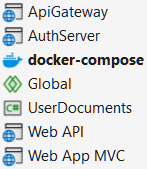
\includegraphics[width=0.4\textwidth]{fig/elenco_progetti.png}
    \caption[Elenco progetti]{Elenco dei progetti che compongono il codice sorgente della soluzione}
\end{figure}

\subsection{Gateway API}
Il progetto \emph{APIGateway} implementa il pattern omonimo nel contesto della soluzione proposta. Si tratta di un microservizio \emph{ASP.NET Core} che funge da SPoA (\emph{Single Point of Access}) per l'architettura, fornendo funzionalità di \emph{reverse proxying} grazie all'impiego del pacchetto \emph{YARP} e di centralizzazione dell'autenticazione con refresh intelligente dei token.

\emph{YARP} (\emph{Yet Another Reverse Proxy}) è un framework open-source per la creazione di proxy HTTP, sviluppato e mantenuto da Microsoft, che consente di instradare le richieste in ingresso verso uno o più servizi backend in modo flessibile e configurabile. Gran parte delle specifiche di instradamento, infatti, sono state definite direttamente come oggetto all'interno nel file di configurazione del progetto .NET (che per default è nominato \emph{appsettings.json}), mentre le richieste di Logout, che implementano una logica più avanzata per l'invalidazione di cookie e token e per il sign out dal contesto dell'Identity, sono state configurate all'interno del middleware nel file di avvio del progetto \emph{Program.cs}.

L'approccio di estrarre le informazioni variabili in un file di configurazione non riguarda soltanto il routing del reverse proxy, ma è adottato in maniera consistente nei progetti .NET dell'intera applicazione, consentendo non solo di mantenere un file di avvio snello e facilmente leggibile, ma anche di centralizzare la gestione delle configurazioni grazie all'elasticità fornita dall'ambiente \emph{.NET}.
Tali dati sono infatti estratti mediante un oggetto \texttt{ConfigurationManager}, che rappresenta un unico punto d'accesso alle configurazioni, dotato di un sistema di priorità e di metodi per lo strong typing dei valori ottenuti. Per accesso con priorità si intende che il \texttt{ConfigurationManager} di un applicazione ASP.NET è in grado di ricercare le configurazioni richieste da più fonti in una gerarchia stabilita, consentendo allo sviluppatore di specificare override diversi in \emph{environment} diversi (sviluppo, testing, produzione) ed eventualmente di iniettare la configurazione come variabili d'ambiente mediante Docker, semplificando notevolmente il deploy in ambienti distribuiti in cui, ad esempio nel caso del gateway API, è necessario specificare all'avvio le informazioni sulla rete in cui il servizio viene installato.

L'altra funzionalità importante fornita dal progetto \emph{APIGateway} è la gestione centralizzata dell'autenticazione e dell'autorizzazione degli utenti, implementando il pattern \emph{Authentication Gateway}.

Al momento di una richiesta da parte di un client, il gateway verifica che l'utente sia autenticato prima che la richiesta raggiunga i microservizi interni e, in caso contrario, lo ridireziona all'apposita interfaccia grafica fornita dal microservizio AuthServer, che analizzeremo in seguito (se la richiesta è programmatica restituisce invece \texttt{Error 401}): una volta autenticato, all'utente sono associati un token JWT (JSON Web Token) e un cookie, che il gateway provvederà ad inoltrare ai microservizi backend e a rinnovare periodicamente in modo trasparente per l'utente: il token JWT e il cookie consentono all'utente di autenticarsi una volta sola (presso il gateway) e restare connesso per l'uso di Web API e client MVC rispettivamente.

\subsection{AuthServer}
Il progetto \emph{AuthServer} descrive il microservizio che fa da Identity Provider per l'applicativo. Utilizza il framework \emph{Duende Identity Server} per implementare e configurare con pochi metodi un servizio di autenticazione completo basato sul protocollo OpenID Connect. Per la gestione di utenti e ruoli si affida invece ad \emph{Identity} con \emph{EntityFramework Core}: grazie alla potenza e l'interazione \emph{seamless} dei framework, in questo progetto la persistenza è stata gestita in maniera potente ed integrata senza dover scrivere una sola riga di codice \emph{SQL} o dover configurare manualmente il database (qui SQLite ospitato su un \emph{named volume Docker}, configurazione accettabile in un ambiente prototipale per motivazioni discusse in precedenza). Si pensi che l'intera configurazione dell'Identity Server con le funzionalità essenziali (2FA, login con provider esterni o email sender sarebbero inutili in un contesto prototipale offline) è stata realizzata con l'invocazione di meno di 7 metodi nell'entrypoint del servizio (\emph{Program.cs}).
\begin{figure}[H]
        \centering
        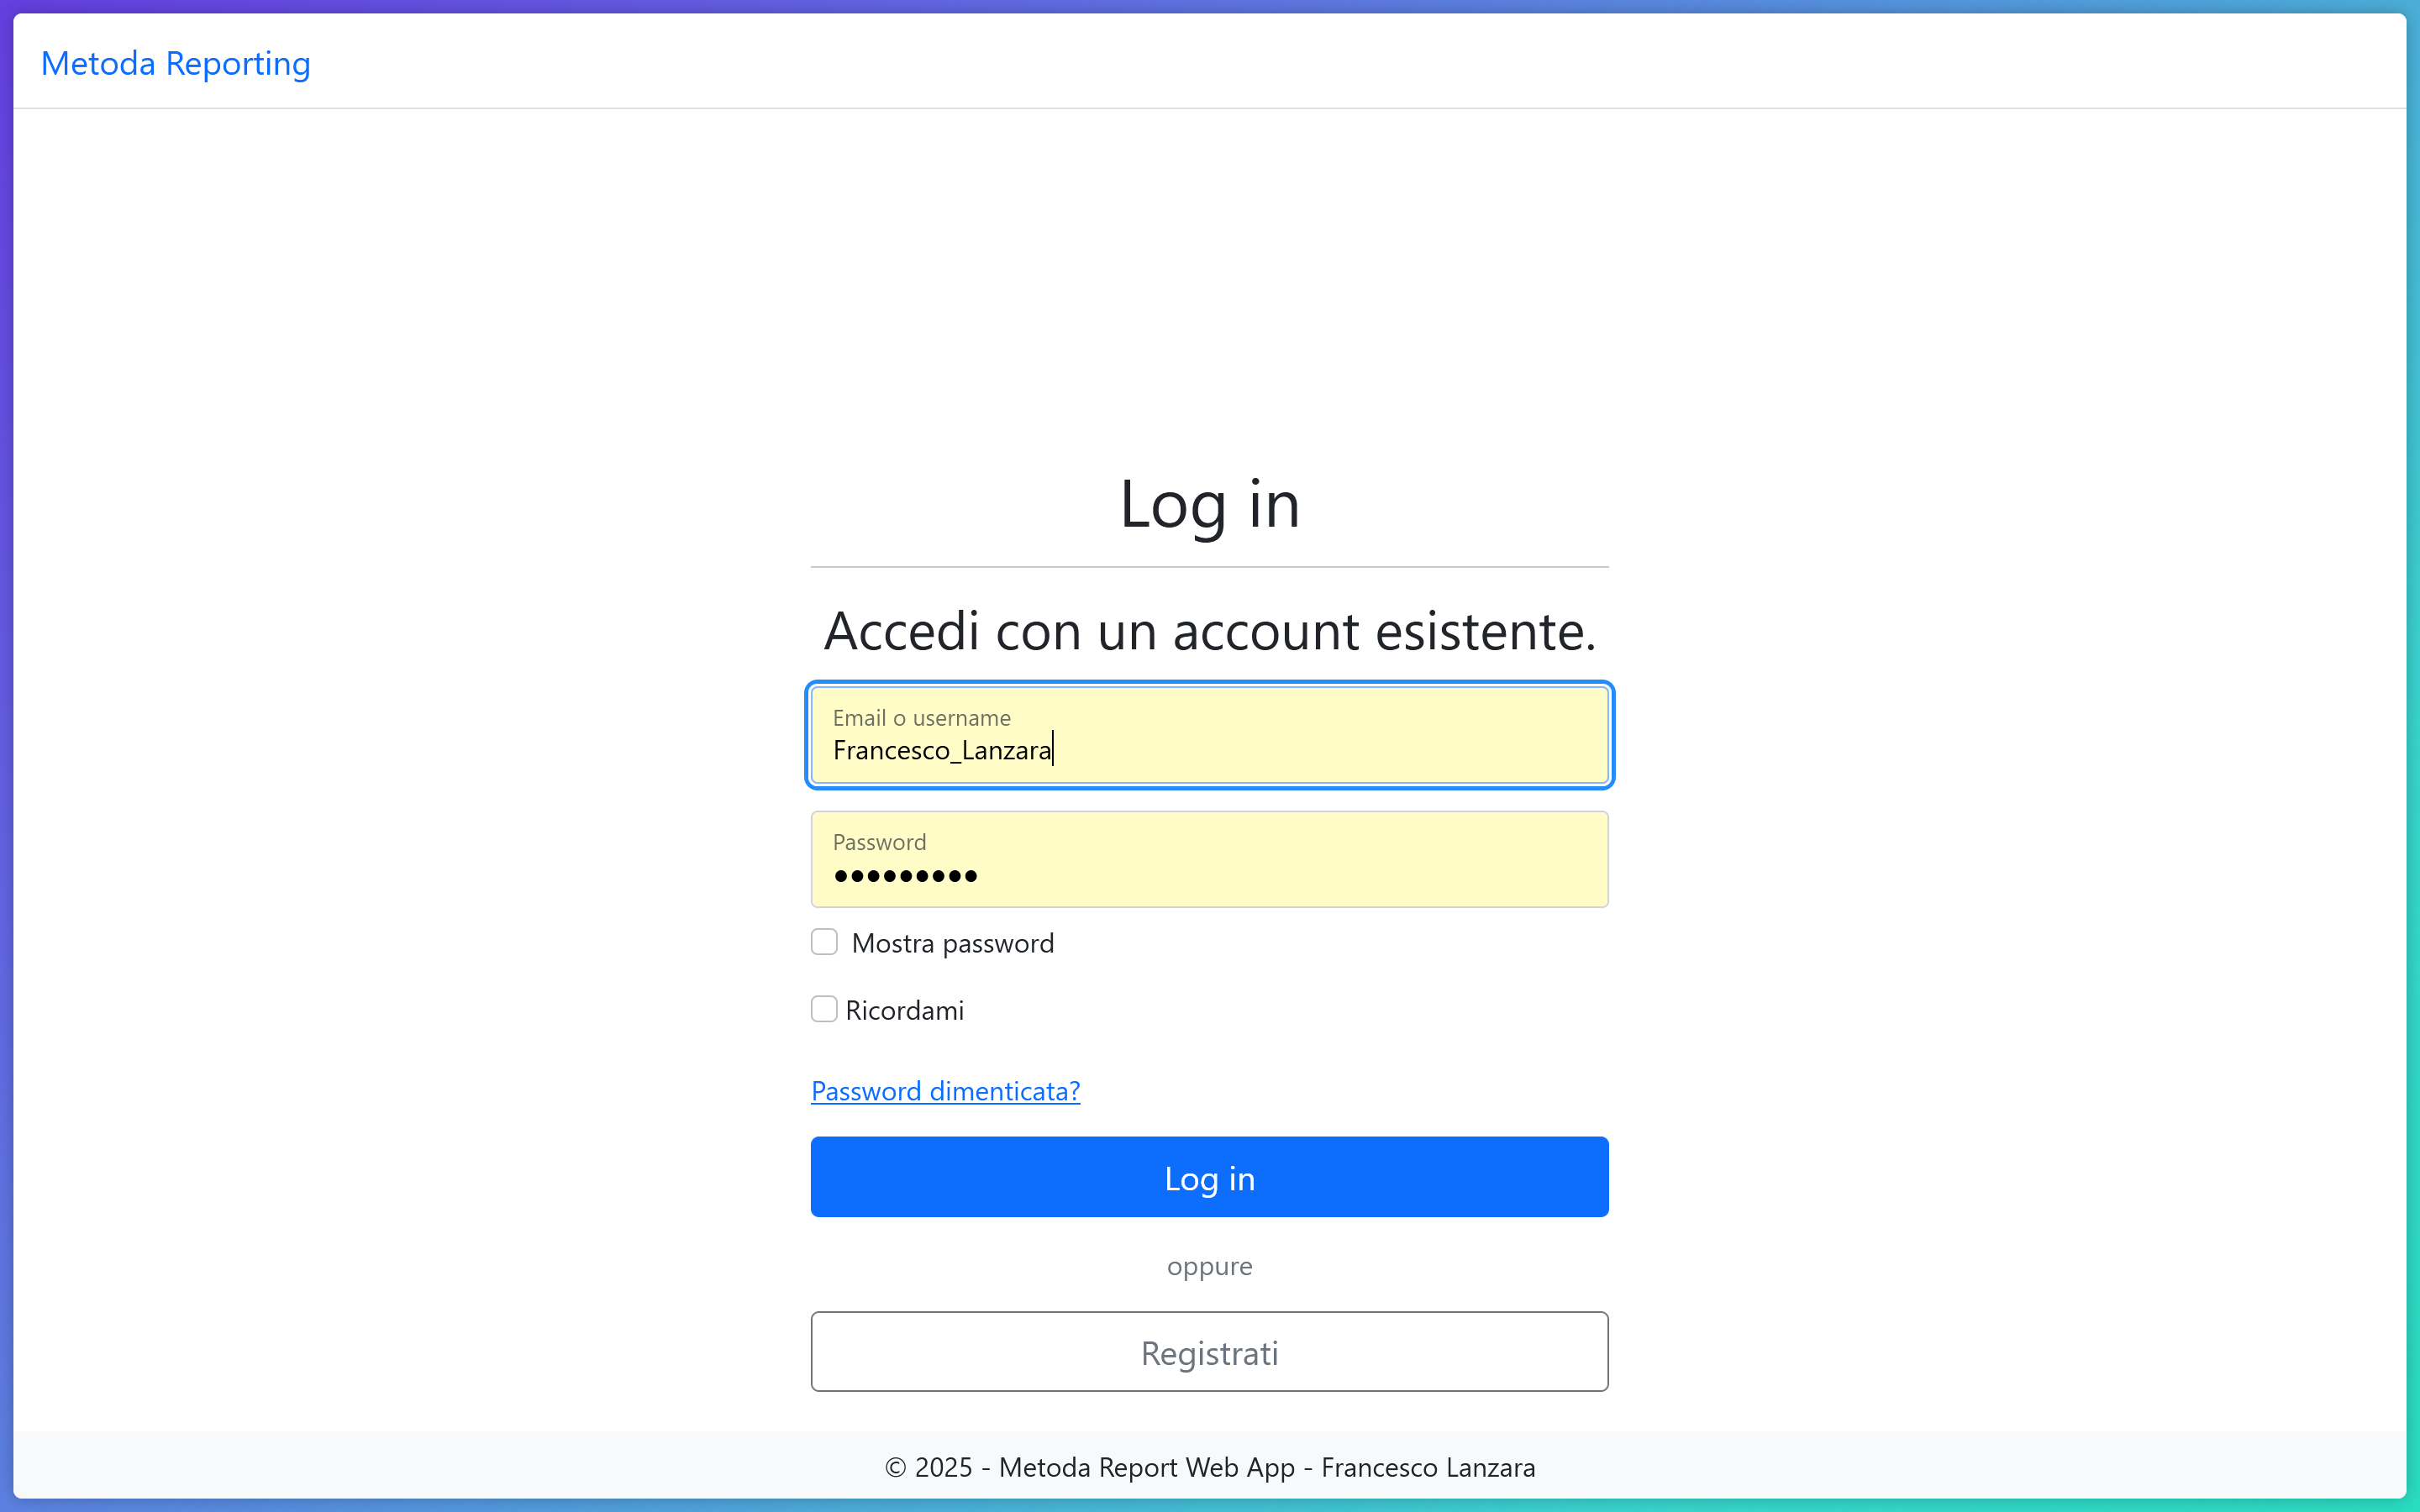
\includegraphics[width=15cm]{fig/screen_login.png}
        \caption[Schermata login]{La schermata di login. Da questa schermata è possibile accedere anche alla registrazione e al recupero della password.}
\end{figure}
Il sistema di scaffolding .NET, che consente la generazione automatica di codice \emph{boilerplate} per la configurazione rapida delle funzionalità offerte dai framework, è stato utilizzato per generare la struttura alla base del rendering delle pagine di accesso, registrazione e gestione del profilo utente, che sono state poi personalizzate per adattarle alle esigenze del progetto e rese gradevoli alla vista con classi del framework \emph{Bootstrap} per \emph{CSS}.
Si tenga conto che nonostante la scelta, analizzata nel capitolo quarto, di implementare l'interfaccia grafica della web app mediante ASP.NET Core MVC, l'implementazione di base generata per interfaccia di autenticazione fa utilizzo della tecnologia \emph{Razor Pages}, che adotta un approccio \emph{MVVC}-like, basato sul concetto di \emph{PageModel}, associando a ogni pagina \texttt{.cshtml} un file \emph{.cs} che ne descrive la logica e il modello: il risultato è una struttura più fluida e meno verbosa che fa largo uso di convenzioni, rendendo semplice implementare funzionalità comuni ma risultando nel complesso meno flessibile di MVC.
\begin{figure}[H]
        \centering
        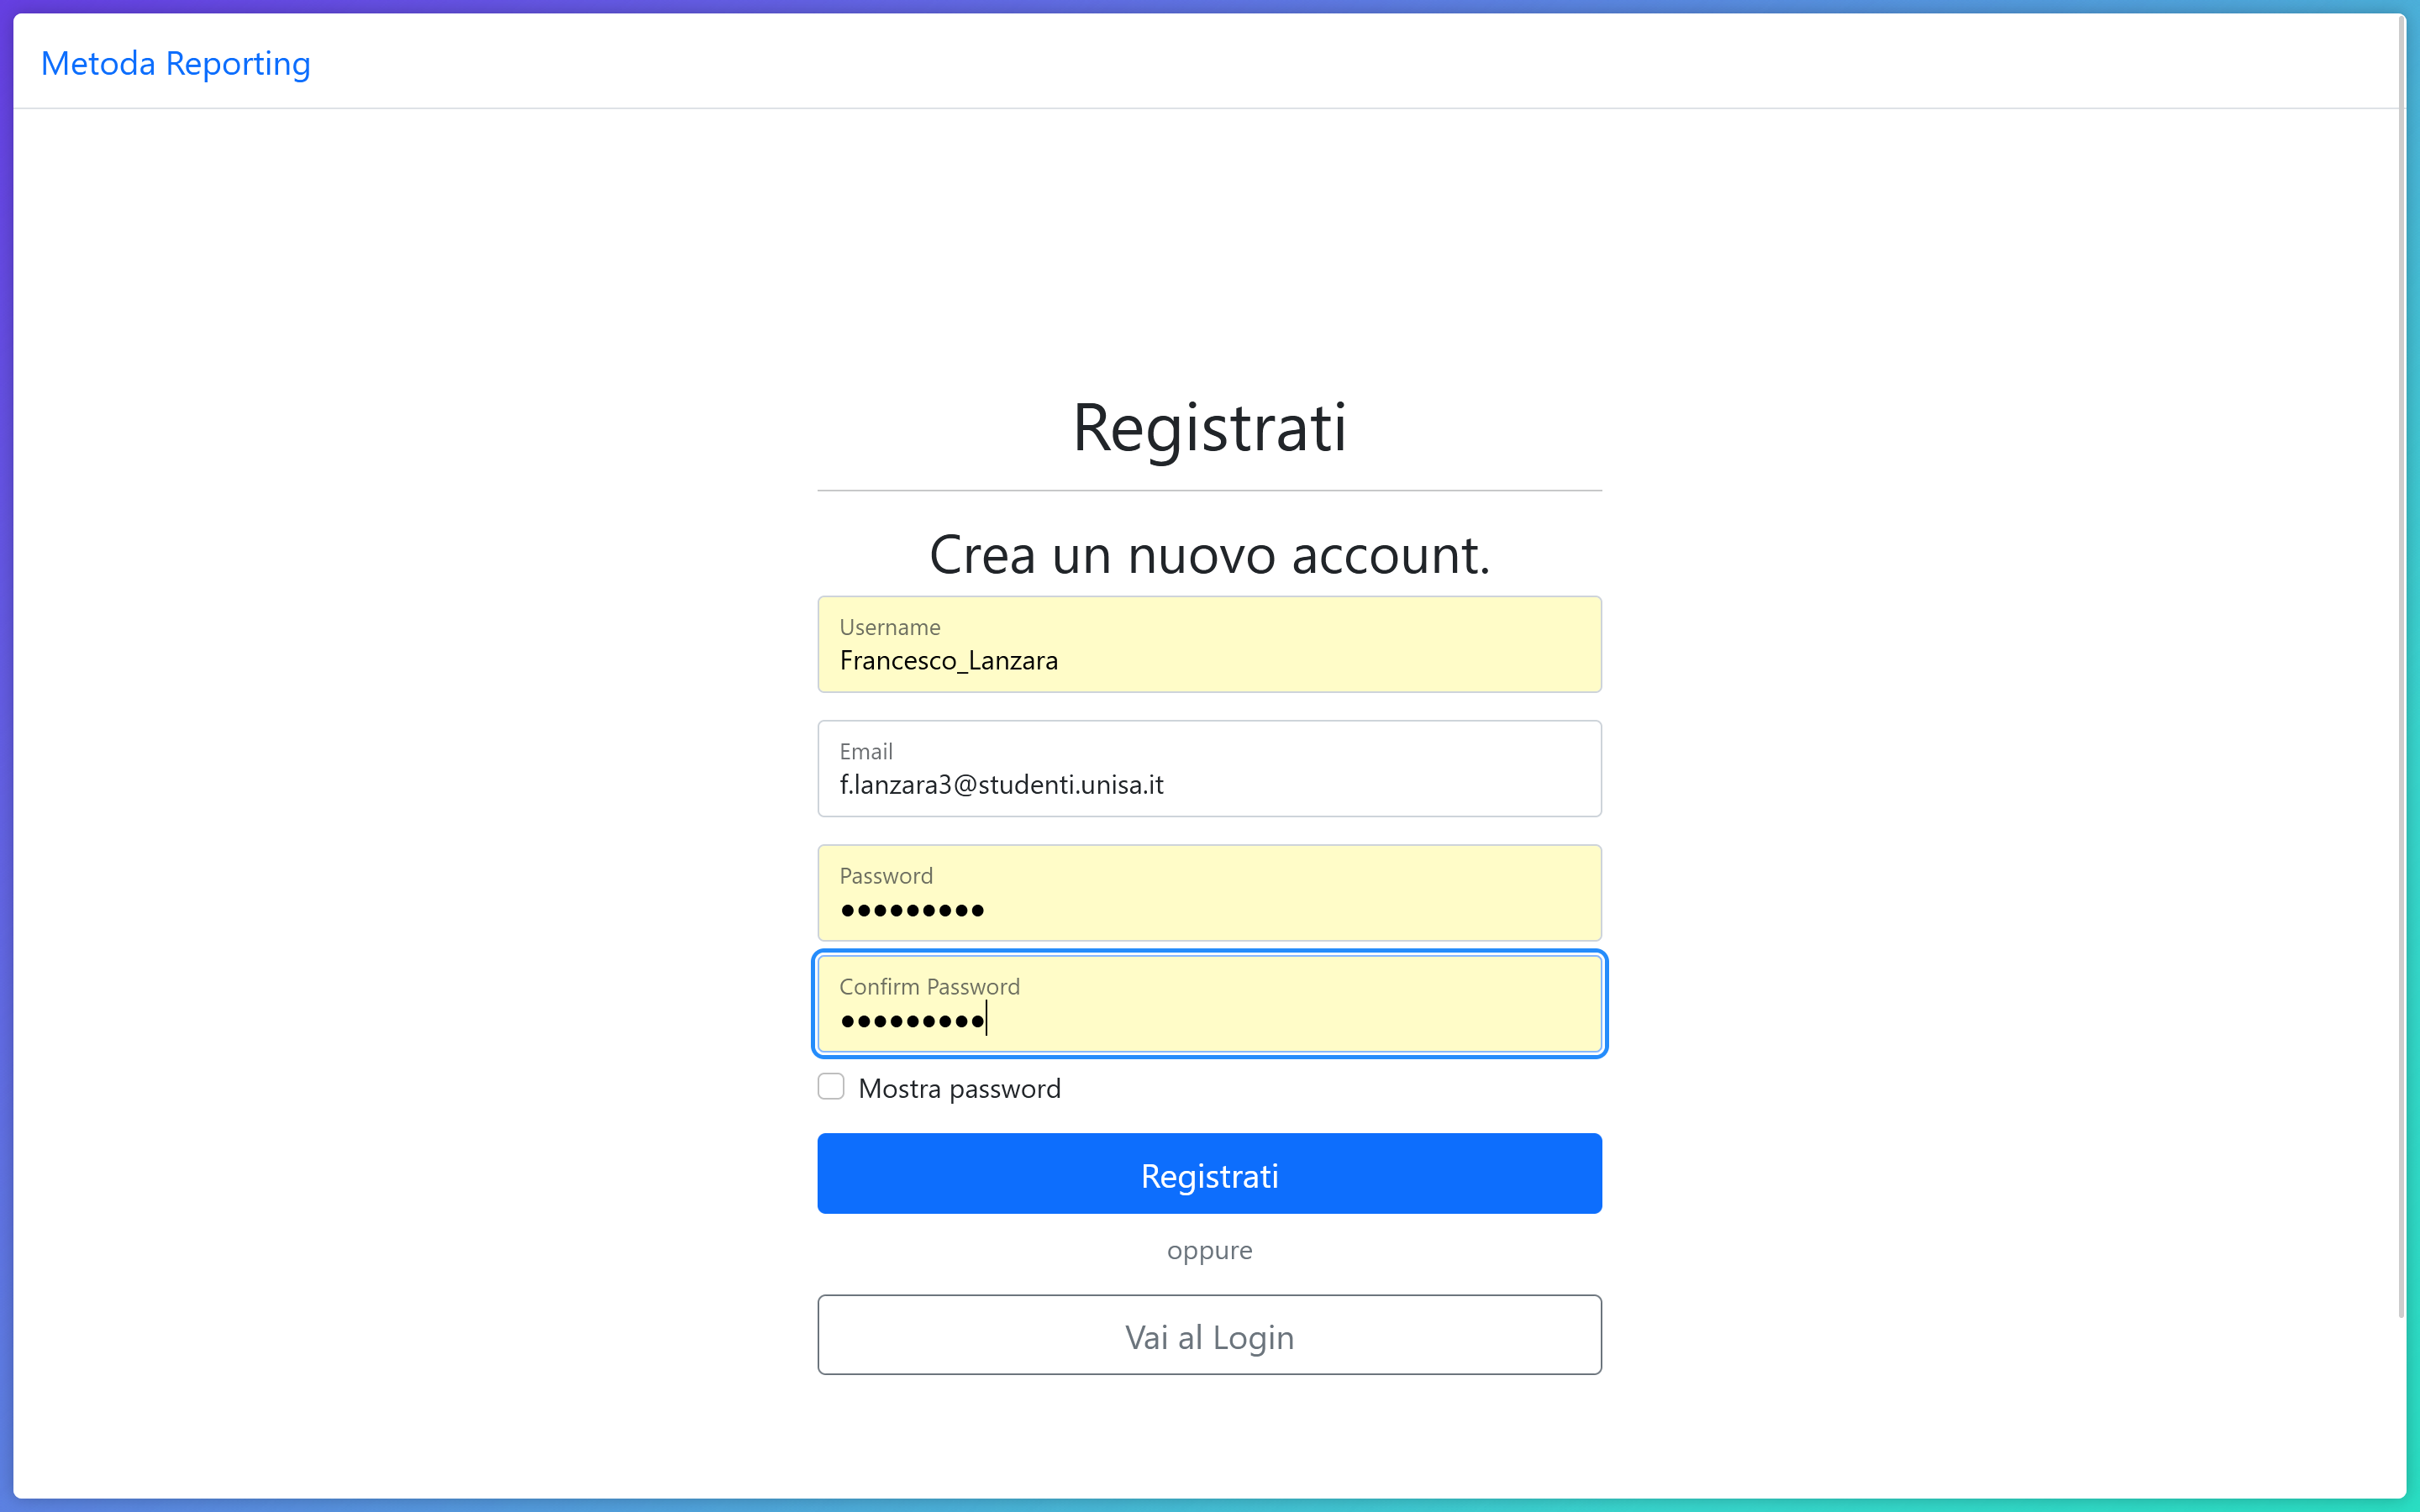
\includegraphics[width=15cm]{fig/screen_register.png}
        \caption[Schermata registrazione]{La schermata di registrazione. Da questa schermata è possibile tornare al login.}
\end{figure}
Dal momento che la logica di autenticazione è gestita internamente lontano dagli occhi dello sviluppatore, il sottoscritto ha ritenuto preferibile mantenere l'implementazione già predisposta, limitandosi a personalizzare aspetto e interazione delle pagine, piuttosto che impiegare tempo per individuare una soluzione alternativa nel tentativo di mantenere coerenza con una scelta implementativa che riguarda un altro microservizio dell'architettura. In un contesto in cui un controllo chiaro sull'implementazione non è ottenibile indipendentemente dalla tecnologia impiegata, il vantaggio principale del pattern MVC viene meno, giustificando ulteriormente la scelta di adottare Blazor per l'AuthServer.

AuthServer si occupa dunque di rispondere alle richieste di autenticazione e fornire le schermate per il login, la registrazione ed altre funzionalità legate all'account, come reset e modifica della password, gestione di altre informazioni del profilo quali recapiti telefonico e mail, logout. Si tenga conto che un utente già autenticato può accedere a queste pagine senza perdere l'accesso, ritornando all'applicazione MVC tramite click sul nome del servizio (estremo sinistro del layout superiore).
Esso espone inoltre gli endpoint necessari per il protocollo OpenID Connect, che consente ai client di autenticare gli utenti e ottenere informazioni sui loro profili in modo sicuro e standardizzato. Tali endpoint sono utilizzati dal gateway API per autenticare gli utenti che tentano di accedere ai microservizi protetti dell'architettura.
L'accesso dell'utente mediante \emph{OpenID Connect} fornisce al browser un cookie di sessione e un codice, che il gateway (punto di accesso dell'utente) utilizza per ottenere un token JWT, inoltrato alla Web API per autorizzare delle richieste.
\begin{figure}[H]
        \centering
        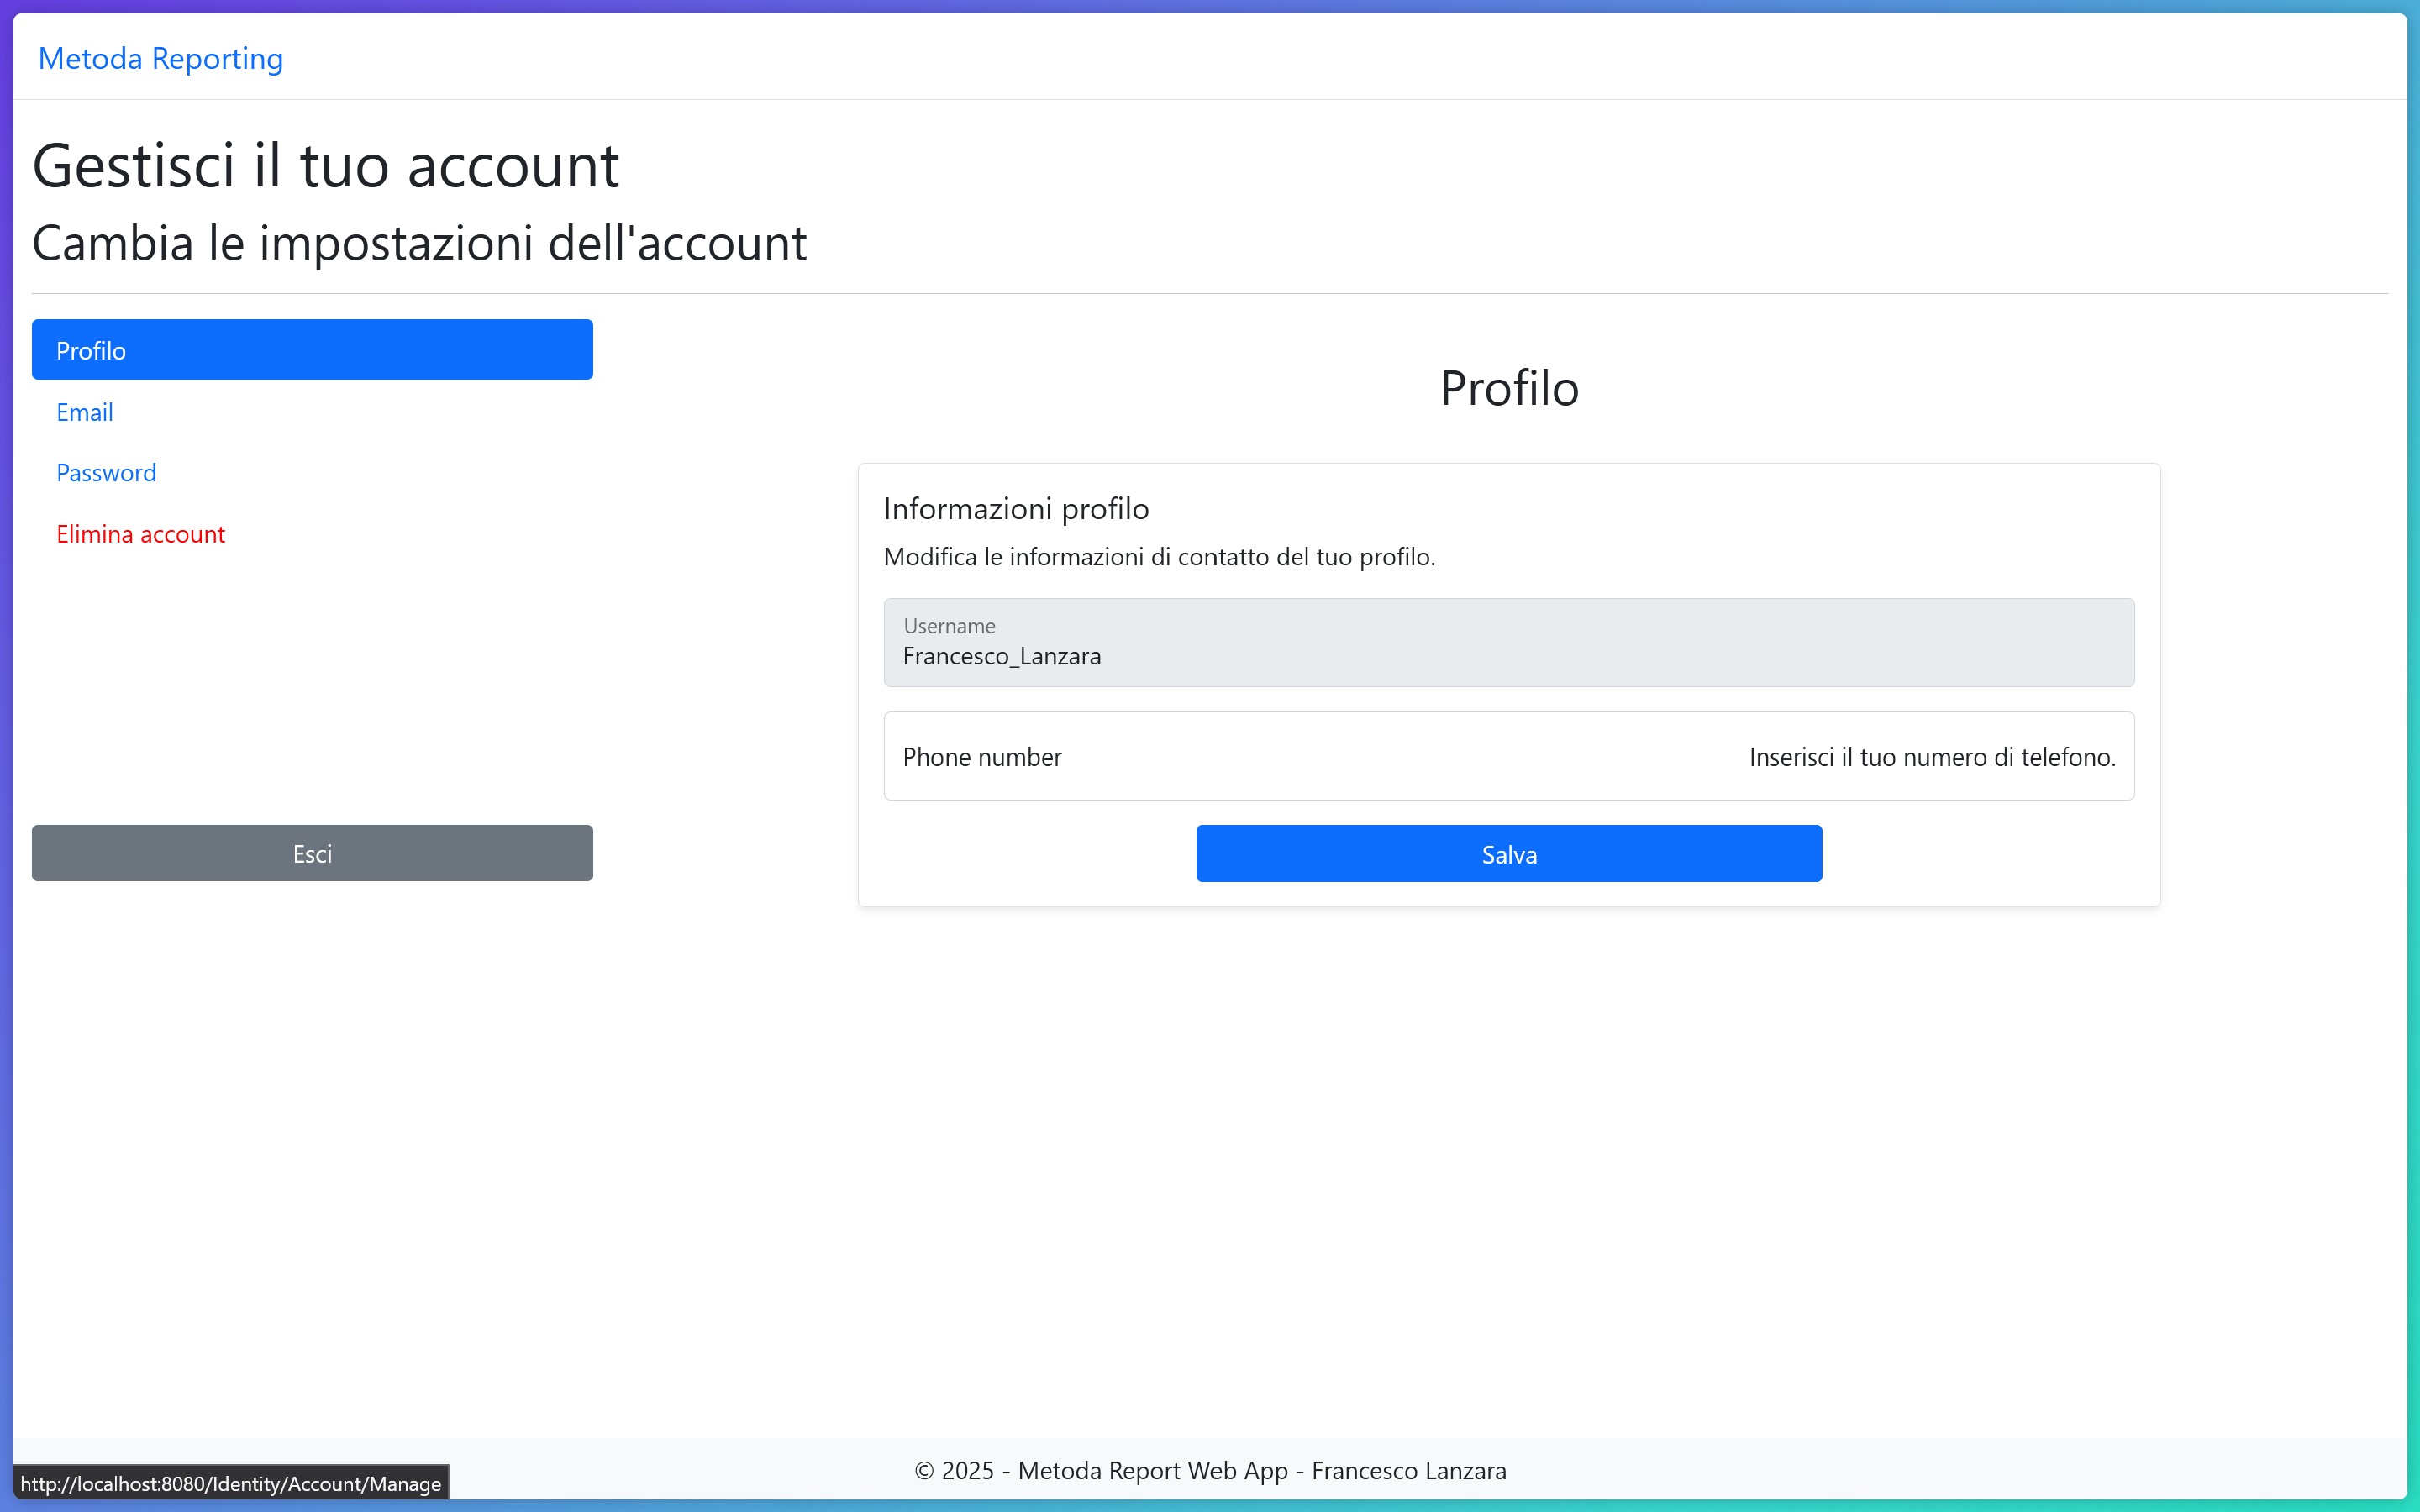
\includegraphics[width=15cm]{fig/screen_manage.png}
        \caption[Schermata gestione utente]{La schermata di gestione account. Contiene le sezioni \emph{profilo, email, password}. E' da questa schermata inoltre che l'utente può effettuare il \emph{logout} ed \emph{eliminare} l'account, i dati a esso assiciati e i documenti da esso generati.}
\end{figure}

In aggiunta a un sistema di refresh automatico dei token, tale sistema consente all'utente di accedere a tutti i microservizi protetti dell'architettura senza preoccuparsi di dover effettuare nuovi login, garantendo un'esperienza utente fluida e sicura che ignora la suddivisione dell'architettura in container distinti.

\subsection{Web API}
Il progetto \emph{WebAPI} implementa il microservizio che espone le API RESTful per la generazione automatica dei report e il loro salvataggio nella sezione dello storage dedicata all'utente: infatti, l'API è protetta dal gateway e pertanto risulta accessibile solo previa autenticazione.
Per realizzare tale servizio si è fatto uso del framework \emph{ASP.NET Core Web API}, che consente di creare API RESTful in modo semplice e veloce.

Come accennato in precedenza, tale microservizio ospita il motore di generazione automatica dei report, i cui moduli sono referenziati nel progetto.
Lo stato persistente è mantenuto su un \emph{named volume Docker}, su cui un database SQLite memorizza i metadati sui documenti generati, associandoli agli utenti mediante il loro \texttt{SubjectId} (identificativo univoco fornito da OpenID Connect), mentre i file stessi sono salvati su file system, con una struttura di cartelle che li organizza per utente e data di creazione. Come prospettiva futura, si dovrebbe aggiungere un sistema di gestione dello spazio utilizzato, come una \emph{policy} di eliminazione automatica dei documenti più vecchi o un limite massimo di spazio utilizzabile per utente, per evitare che lo storage cresca indefinitamente.

Un Controller API astratto implementa, tra gli altri, i due metodi di base necessari alla generazione dei documenti, per l'esportazione rispettivamente in formati PDF ed Excel (\texttt{.xlsm}), che possono essere chiamati dai controller concreti apponendo i tipi parametrici adeguati (tra quelli disponibili del motore di reportistica) al fine di specificare categoria di report e \emph{data source} (per il testing sono state utilizzate classi statiche di tipo \texttt{-FakeData} predisposte dal modulo di test del motore di reportistica) e ottenere il report desiderato con un approccio semplice e modulare. Un ulteriore metodo è messo a disposizione per il \emph{retrieval} dei documenti precedentemente generati dall'utente e presenti in storage: come vedremo a breve, tale metodo è utilizzato dal client MVC per popolare una lista di documenti recenti con link predisposti per il download degli stessi.

La generazione dei documenti avviene in modo asincrono, con la creazione di un nuovo task per ogni richiesta, in modo da non bloccare il thread principale del server e consentire la gestione di più richieste contemporaneamente. Una volta completata la generazione, il documento viene salvato nello storage e i metadati vengono aggiornati nel database.

Essendo il principale incaricato della generazione dei report, il microservizio Web API istanzia un Hub SignalR per l'aggiornamento in tempo reale sullo stato di generazione dei report. In questo modo, quando la generazione di un documento viene richiesta dal client MVC, esso si iscrive all'hub; il controller della Web API associa all'oggetto report un \texttt{ReportProgress}, classe del motore di reportistica, che in maniera nativa consente di associare una \emph{callback} al progresso nella fase di generazione. Impostando come callback la procedura di emissione di un evento SignalR all'utente, questo può visualizzare a schermo notifiche in tempo reale sulla percentuale di avanzamento dell'operazione richiesta.

Tutti i controller concreti espongono endpoint \texttt{GET} alla route URL \url{{dominio}/api/{CategoriaReport}/{pdf|excel}}, e si limitano a restituire in maniera asincrona il risultato del metodo generico ereditato, specificando i parametri di tipo adeguati. Ad esempio, per generare un report di tipo \emph{MonthlyReport} (Report Analitico per Controparte) in formato PDF, il client deve invocare l'endpoint
\url{{dominio}/api/MonthlyReport/pdf}, ottenendo in risposta il file generato.

Infine, \emph{WebAPI} utilizza il progetto condiviso \emph{UserDocuments}, che definisce il modello di dati per i documenti generati e i metadati ad essi associati, in modo da poter interagire con il database SQLite in modo tipizzato e sicuro.

\subsection{Client MVC}









